% \documentclass[border=10pt]{standalone}
% \usepackage{tikz}
% \begin{document}
% \begin{tikzpicture}[sibling distance=10em,
%   every node/.style = {shape=rectangle, rounded corners,
%     align=center}]]
%   \node [draw] {$(x-x_0)(x-x_1)\ldots(x-x_{n-1})$}
%     child { node {$\vdots$}
%       child { node [draw] {$(x-x_0)$}}
%       child { node [draw] {$(x-x_1)$}}}
%     child { node {$\vdots$}
%       child { node {aligned at}
%         child { node {relation sign} }
%         child { node {several places} }
%         child { node {center} } }
%       child { node {first left,\\centered,\\last right} } };
% \end{tikzpicture}
% \end{document}

\documentclass[border=10pt]{standalone}
\usepackage{fancybox}
\usepackage{tikz}

\title{MergeSort-RecursionTree}
\author{Manuel Kirsch}
\date{}
\begin{document}

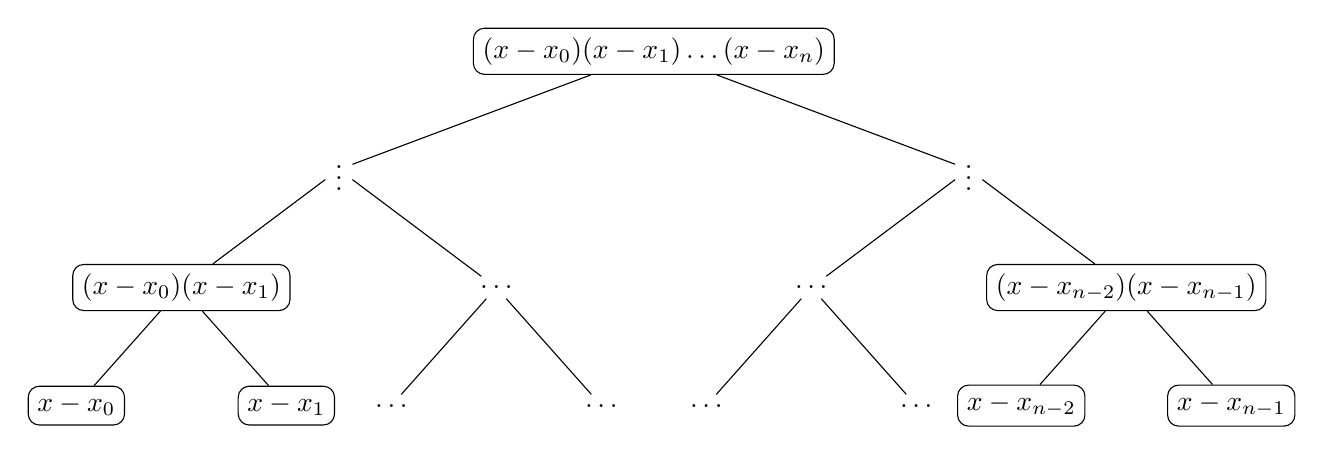
\begin{tikzpicture}[level/.style={sibling distance=80mm/#1},
  every node/.style = {shape=rectangle, rounded corners,
     align=center}]
\node [draw] (z){$(x-x_0)(x-x_1)\ldots(x-x_n)$}
  child {node [] (a) {$\vdots$}
    child {node [draw] (b) {$(x-x_0)(x-x_1)$}
      child {node [draw] {$x-x_0$}}
      child {node [draw] {$x-x_1$}}
    }
    child {node (g) {$\ldots$}
      child {node {$\ldots$}}
      child {node {$\ldots$}}
    }
  }
  child {node [] (j) {$\vdots$}
    child {node (k) {$\ldots$}
      child {node {$\ldots$}}
      child {node {$\ldots$}}
    }
  child {node [draw] (l) {$(x-x_{n-2})(x-x_{n-1})$}
    child {node [draw] {$x-x_{n-2}$}}
    child {node [draw] (c){$x-x_{n-1}$}}
  }
};
\end{tikzpicture}

\end{document}